% This file was created by matlab2tikz.
%
%The latest updates can be retrieved from
%  http://www.mathworks.com/matlabcentral/fileexchange/22022-matlab2tikz-matlab2tikz
%where you can also make suggestions and rate matlab2tikz.
%
\definecolor{mycolor1}{rgb}{0.00000,0.44700,0.74100}%
\definecolor{mycolor2}{rgb}{0.85000,0.32500,0.09800}%
\definecolor{mycolor3}{rgb}{0.92900,0.69400,0.12500}%
\definecolor{mycolor4}{rgb}{0.49400,0.18400,0.55600}%
%
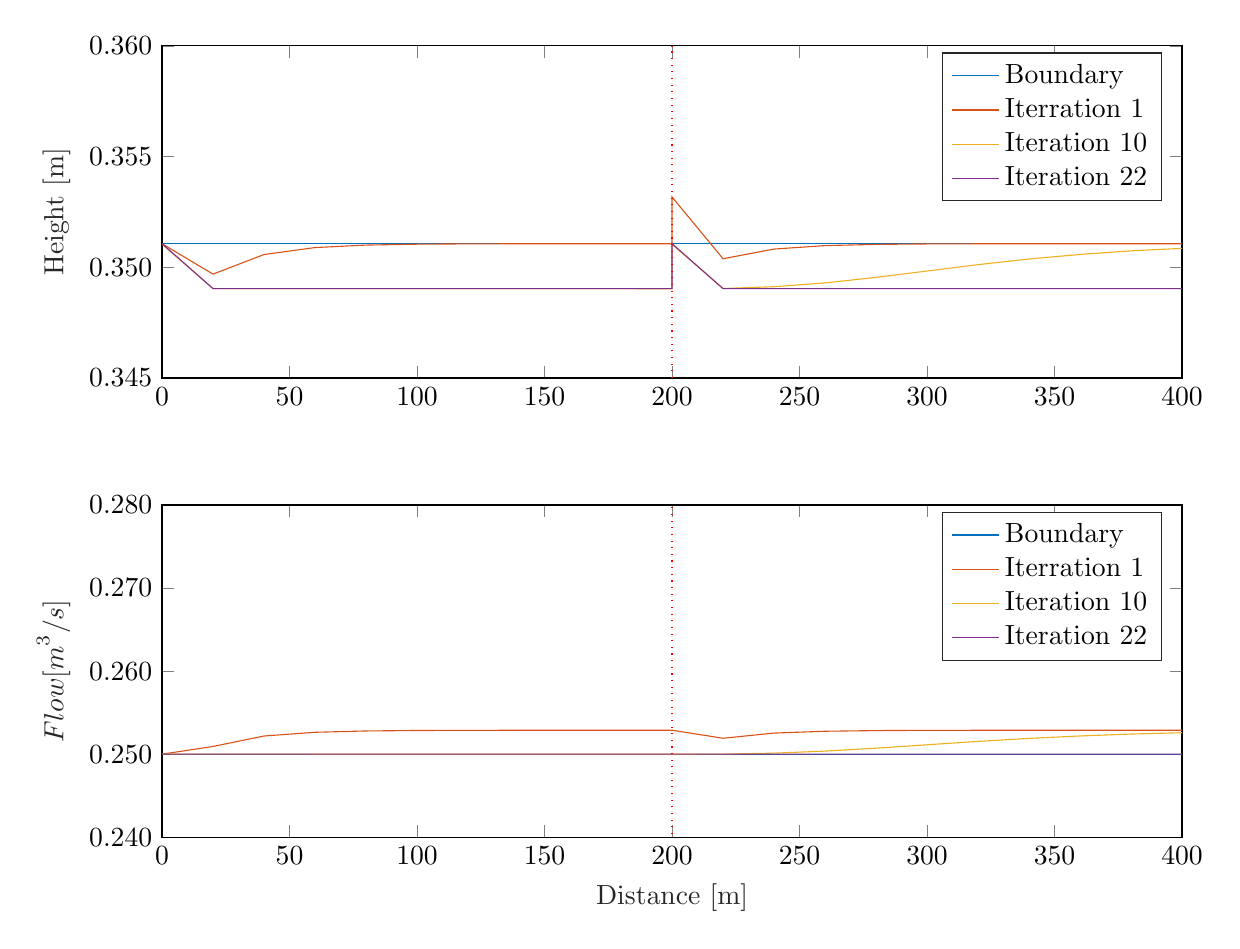
\begin{tikzpicture}

\begin{axis}[%
width=5.1in,
height=1.661in,
at={(2.08in,3.154in)},
scale only axis,
xmin=0,
xmax=400,
xlabel style={font=\color{white!15!black}},
%xlabel={Distance [m]},
ymin=0.345,
ymax=0.36,
ylabel style={font=\color{white!15!black}},
ylabel={Height [m]},
axis background/.style={fill=white},
y tick label style={
        /pgf/number format/.cd,
            fixed,
            fixed zerofill,
            precision=3,
        /tikz/.cd  },
title style={font=\bfseries},
%title={Curvefit},
legend style={legend cell align=left, align=left, draw=white!15!black}
]
\addplot [color=mycolor1]
  table[row sep=crcr]{%
0	0.351064698342896\\
200	0.351064698342896\\
400	0.351064698342896\\
};
\addlegendentry{Boundary}

\addplot [color=mycolor2]
  table[row sep=crcr]{%
0	0.351064698342896\\
20	0.349690425371762\\
40	0.350575480853252\\
60	0.350890269562512\\
80	0.351002475151802\\
100	0.351042501121412\\
120	0.351056775490292\\
140	0.351061870368596\\
200	0.351064571998904\\
200	0.35317394090697\\
220	0.350385544412916\\
240	0.350822634043709\\
260	0.350978353573737\\
280	0.351033892189093\\
300	0.351053708086965\\
320	0.351060775514213\\
360	0.351064199156951\\
400	0.351064634411387\\
};
\addlegendentry{Iterration 1}

\addplot [color=mycolor3]
  table[row sep=crcr]{%
0	0.351046566681021\\
20	0.349036521512801\\
180	0.349035279823624\\
200	0.349026739276496\\
200	0.35103637024929\\
220	0.349041213224552\\
240	0.349123089812394\\
260	0.349294685503196\\
280	0.349543083040601\\
320	0.350118505975786\\
340	0.350374059351282\\
360	0.350579188303925\\
380	0.350742011157763\\
400	0.350854227957257\\
};
\addlegendentry{Iteration 10}

\addplot [color=mycolor4]
  table[row sep=crcr]{%
0	0.351064698342952\\
20	0.349036521507401\\
200	0.349036522122788\\
200	0.351064698342952\\
220	0.349036521507401\\
400	0.349036532325727\\
};
\addlegendentry{Iteration 22}

\addplot [color=red, dotted, forget plot]
  table[row sep=crcr]{%
200	0.344999999999999\\
200	0.360000000000014\\
};
\end{axis}

\begin{axis}[%
width=5.1in,
height=1.661in,
at={(2.08in,0.858in)},
scale only axis,
xmin=0,
xmax=400,
xlabel style={font=\color{white!15!black}},
xlabel={Distance [m]},
ymin=0.24,
ymax=0.28,
ylabel style={font=\color{white!15!black}},
ylabel={$\text{Flow [m}^\text{3}\text{/s]}$},
y tick label style={
        /pgf/number format/.cd,
            fixed,
            fixed zerofill,
            precision=3,
        /tikz/.cd  },
axis background/.style={fill=white},
legend style={legend cell align=left, align=left, draw=white!15!black}
]
\addplot [color=mycolor1]
  table[row sep=crcr]{%
0	0.25\\
200	0.25\\
400	0.25\\
};
\addlegendentry{Boundary}

\addplot [color=mycolor2]
  table[row sep=crcr]{%
0	0.25\\
20	0.250927811672625\\
40	0.252185983866809\\
60	0.252634142815168\\
80	0.252793964154193\\
100	0.252850978285323\\
140	0.25287858109607\\
200	0.252882427974328\\
220	0.251915745479664\\
240	0.252537816935785\\
260	0.252759602617687\\
280	0.252838721204057\\
300	0.252866948997394\\
340	0.25288061725945\\
400	0.252882518538513\\
};
\addlegendentry{Iterration 1}

\addplot [color=mycolor3]
  table[row sep=crcr]{%
0	0.25\\
200	0.249986131352046\\
220	0.25000665171865\\
240	0.250122746526756\\
260	0.250366131411454\\
280	0.25071862987113\\
320	0.251536029676629\\
340	0.251899416890069\\
360	0.252191266279397\\
380	0.252423028186058\\
400	0.252582810584272\\
};
\addlegendentry{Iteration 10}

\addplot [color=mycolor4]
  table[row sep=crcr]{%
0	0.25\\
200	0.25\\
400	0.250000020948733\\
};
\addlegendentry{Iteration 22}

\addplot [color=red, dotted, forget plot]
  table[row sep=crcr]{%
200	0.22999999999999\\
200	0.300000000000011\\
};
\end{axis}
\end{tikzpicture}%